% Options for packages loaded elsewhere
\PassOptionsToPackage{unicode}{hyperref}
\PassOptionsToPackage{hyphens}{url}
\PassOptionsToPackage{dvipsnames,svgnames,x11names}{xcolor}
%
\documentclass[
  letterpaper,
]{article}

\usepackage{amsmath,amssymb}
\usepackage{lmodern}
\usepackage{iftex}
\ifPDFTeX
  \usepackage[T1]{fontenc}
  \usepackage[utf8]{inputenc}
  \usepackage{textcomp} % provide euro and other symbols
\else % if luatex or xetex
  \usepackage{unicode-math}
  \defaultfontfeatures{Scale=MatchLowercase}
  \defaultfontfeatures[\rmfamily]{Ligatures=TeX,Scale=1}
\fi
% Use upquote if available, for straight quotes in verbatim environments
\IfFileExists{upquote.sty}{\usepackage{upquote}}{}
\IfFileExists{microtype.sty}{% use microtype if available
  \usepackage[]{microtype}
  \UseMicrotypeSet[protrusion]{basicmath} % disable protrusion for tt fonts
}{}
\makeatletter
\@ifundefined{KOMAClassName}{% if non-KOMA class
  \IfFileExists{parskip.sty}{%
    \usepackage{parskip}
  }{% else
    \setlength{\parindent}{0pt}
    \setlength{\parskip}{6pt plus 2pt minus 1pt}}
}{% if KOMA class
  \KOMAoptions{parskip=half}}
\makeatother
\usepackage{xcolor}
\setlength{\emergencystretch}{3em} % prevent overfull lines
\setcounter{secnumdepth}{3}
% Make \paragraph and \subparagraph free-standing
\ifx\paragraph\undefined\else
  \let\oldparagraph\paragraph
  \renewcommand{\paragraph}[1]{\oldparagraph{#1}\mbox{}}
\fi
\ifx\subparagraph\undefined\else
  \let\oldsubparagraph\subparagraph
  \renewcommand{\subparagraph}[1]{\oldsubparagraph{#1}\mbox{}}
\fi


\providecommand{\tightlist}{%
  \setlength{\itemsep}{0pt}\setlength{\parskip}{0pt}}\usepackage{longtable,booktabs,array}
\usepackage{calc} % for calculating minipage widths
% Correct order of tables after \paragraph or \subparagraph
\usepackage{etoolbox}
\makeatletter
\patchcmd\longtable{\par}{\if@noskipsec\mbox{}\fi\par}{}{}
\makeatother
% Allow footnotes in longtable head/foot
\IfFileExists{footnotehyper.sty}{\usepackage{footnotehyper}}{\usepackage{footnote}}
\makesavenoteenv{longtable}
\usepackage{graphicx}
\makeatletter
\def\maxwidth{\ifdim\Gin@nat@width>\linewidth\linewidth\else\Gin@nat@width\fi}
\def\maxheight{\ifdim\Gin@nat@height>\textheight\textheight\else\Gin@nat@height\fi}
\makeatother
% Scale images if necessary, so that they will not overflow the page
% margins by default, and it is still possible to overwrite the defaults
% using explicit options in \includegraphics[width, height, ...]{}
\setkeys{Gin}{width=\maxwidth,height=\maxheight,keepaspectratio}
% Set default figure placement to htbp
\makeatletter
\def\fps@figure{htbp}
\makeatother

\makeatletter
\makeatother
\makeatletter
\makeatother
\makeatletter
\@ifpackageloaded{caption}{}{\usepackage{caption}}
\AtBeginDocument{%
\ifdefined\contentsname
  \renewcommand*\contentsname{Table of contents}
\else
  \newcommand\contentsname{Table of contents}
\fi
\ifdefined\listfigurename
  \renewcommand*\listfigurename{List of Figures}
\else
  \newcommand\listfigurename{List of Figures}
\fi
\ifdefined\listtablename
  \renewcommand*\listtablename{List of Tables}
\else
  \newcommand\listtablename{List of Tables}
\fi
\ifdefined\figurename
  \renewcommand*\figurename{Figure}
\else
  \newcommand\figurename{Figure}
\fi
\ifdefined\tablename
  \renewcommand*\tablename{Table}
\else
  \newcommand\tablename{Table}
\fi
}
\@ifpackageloaded{float}{}{\usepackage{float}}
\floatstyle{ruled}
\@ifundefined{c@chapter}{\newfloat{codelisting}{h}{lop}}{\newfloat{codelisting}{h}{lop}[chapter]}
\floatname{codelisting}{Listing}
\newcommand*\listoflistings{\listof{codelisting}{List of Listings}}
\makeatother
\makeatletter
\@ifpackageloaded{caption}{}{\usepackage{caption}}
\@ifpackageloaded{subcaption}{}{\usepackage{subcaption}}
\makeatother
\makeatletter
\@ifpackageloaded{tcolorbox}{}{\usepackage[many]{tcolorbox}}
\makeatother
\makeatletter
\@ifundefined{shadecolor}{\definecolor{shadecolor}{rgb}{.97, .97, .97}}
\makeatother
\makeatletter
\makeatother
\ifLuaTeX
  \usepackage{selnolig}  % disable illegal ligatures
\fi
\usepackage[]{biblatex}
\addbibresource{../../../../references.bib}
\IfFileExists{bookmark.sty}{\usepackage{bookmark}}{\usepackage{hyperref}}
\IfFileExists{xurl.sty}{\usepackage{xurl}}{} % add URL line breaks if available
\urlstyle{same} % disable monospaced font for URLs
\hypersetup{
  pdftitle={Linux Primeros Pasos},
  pdfauthor={Edison Achalma Mendoza},
  colorlinks=true,
  linkcolor={blue},
  filecolor={Maroon},
  citecolor={Blue},
  urlcolor={Blue},
  pdfcreator={LaTeX via pandoc}}

\title{Linux Primeros Pasos}
\usepackage{etoolbox}
\makeatletter
\providecommand{\subtitle}[1]{% add subtitle to \maketitle
  \apptocmd{\@title}{\par {\large #1 \par}}{}{}
}
\makeatother
\subtitle{Una guía para principiantes en Linux}
\author{Edison Achalma Mendoza}
\date{5/2/23}

\begin{document}
\maketitle
\ifdefined\Shaded\renewenvironment{Shaded}{\begin{tcolorbox}[sharp corners, interior hidden, borderline west={3pt}{0pt}{shadecolor}, enhanced, breakable, frame hidden, boxrule=0pt]}{\end{tcolorbox}}\fi

\renewcommand*\contentsname{Contenidos}
{
\hypersetup{linkcolor=}
\setcounter{tocdepth}{2}
\tableofcontents
}
LINUX\\
primeros pasos como usuario

SISTEMAS OPERATIVOS

SISTEMA OPERATIVO es el conjunto de programas que proporciona los
mecanismos y reglas básicas de funcionamiento para acceder a los
recursos del ordenador de forma adecuada, especialmente a todos los
dispositivos periféricos.

\begin{itemize}
\tightlist
\item
  \textbf{MS-DOS}
\item
  \textbf{WINDOWS}
\item
  \textbf{Mac-OS}
\item
  \textbf{UNIX}~(Grandes máquinas)~------~~\textbf{LINUX}~(PCs)
\end{itemize}

Tipos de programas:

\begin{itemize}
\tightlist
\item
  \textbf{Programas de Control}: Gestión de software y hardware, p.e.
  colas de impresión, etc.
\item
  \textbf{Utilidades del sistema}: editores de texto, compiladores,
  gestión de correo, etc.
\end{itemize}

ORIGEN Y DESARROLLO DE LINUX

\begin{itemize}
\tightlist
\item
  Creado por~\textbf{Linus Torvalds}~en 1991. Inspirado
  en~\textbf{UNIX}.
\item
  Sistema~\textbf{multiusuario}~y~\textbf{multitarea}.
\item
  Desarrollado por miles de programadores en la red.
\item
  Filosofía~\textbf{GNU}. Libre distribución bajo~\textbf{GPL}~(General
  Public License).
\item
  No garantizado. Flexible, estable y barato.
\item
  Al principio no era fácil de usar, porque estaba pensado para
  programadores.
\item
  Cada vez se desarrollan más aplicaciones y utilidades pensando en
  usuarios no programadores, para facilitar el uso de INTERNET y
  competir con WINDOWS.
\end{itemize}

\textbf{Distribuciones}: Núcleo (\textbf{Kernel}) de Linux +~
Aplicaciones y Utilidades para un grupo específico de usuarios

\begin{itemize}
\tightlist
\item
  Algunas distribuciones son gratuitas y otras no.
\item
  Algunas de las distribuciones están mantenidas por empresas
  comerciales (ej. RedHat, Fedora, openSUSE, Ubuntu), y otras son
  mantenidas por una comunidad de programadores (ej. Debian).
\item
  Normalmente se obtiene una distribución descargándola de Internet.
\item
  Distribuciones mas usadas:

  \begin{itemize}
  \tightlist
  \item
    \textbf{Debian}
  \item
    \textbf{Slackware}
  \item
    \textbf{SUSE}
  \item
    \textbf{Caldera}
  \item
    \textbf{Red Hat Enterprise Linux}(comercial)
  \item
    \textbf{Fedora Project}~(basada en RedHat)
  \item
    \textbf{Mandriva}~(basada en RedHat)
  \item
    \textbf{Ubuntu}~(basada en Debian)
  \item
    \textbf{Guadalinex}~(basado en Debian, promovido por la Junta de
    Andalucía)
  \end{itemize}
\end{itemize}

PRIMEROS PASOS

\textbf{ARRANQUE DEL SISTEMA}

\begin{itemize}
\tightlist
\item
  \textbf{LILO o GRUB:}~programa que se encarga de arrancar el S.O.
  deseado por el usuario cuando coexisten Windows y Linux
\end{itemize}

\textbf{INICIO DE UNA SESIÓN DE USUARIO}

\begin{itemize}
\tightlist
\item
  \textbf{Login}:Nombre del usuario.
\item
  \textbf{Password}: Contraseña secreta de acceso privado de cada
  usuario. (Sólo aparecen asteriscos cuando se teclea)
\end{itemize}

\textbf{ELECCIÓN DE PASSWORDS}

La utilización de passwords está hoy en día extendida a muchos aspectos
de la vida cotidiana, no sólo a la utilización de máquinas compartidas.

La elección de un~\textbf{password seguro}~es tanto más crucial cuanto
mayor sea la importancia de lo que ``protege'': cuentas bancarias,
messenger, cuenta de e-mail, reserva de biletes de tren, etc.

Passwords no seguros pueden ser averiguados por programas especializados
en un tiempo inferior a 1 segundo (por ejemplo para una palabra de
diccionario) o en pocas horas (passwords de hasta 6 caracteres formados
por letras mayúsculas, minúsculas y números).

Variantes del tipo sustituir A por 4 , la E por un 3, o la I por un 1
están ya incorporadas en los crackers.

Recomendación para passwords importantes:

\begin{itemize}
\tightlist
\item
  Utilizar passwords cuanto más largos mejor, al menos de 6 caracteres
  (mejor 8)
\item
  Utilizar letras mayúsculas, minúsculas, números y caracteres
  especiales~ como~\textbf{! '' \$ \% \& / ( ) = ? ¿}
\item
  El tiempo para crackear un password así con 8 caracteres es de 39 años
  !!!
\end{itemize}

Lo que NO debes hacer con un password:

\begin{itemize}
\tightlist
\item
  Apuntarlo en un post-it y pegarlo en la pantalla
\item
  Decírselo a cualquiera
\item
  Usar palabras de un diccionario, ni siquiera concatenadas
  (megustaminovio)
\item
  Usar passwords de menos de 6 caracteres
\item
  Llevar las claves de tarjetas y los passwords de las cuentas bancarias
  por internet en la cartera, o en una agenda en el bolso.
\end{itemize}

\textbf{EL PROBLEMA DE LOS BUENOS PASSWORDS ES ACORDARSE DE ELLOS: aqui
tienes un truco}

Piensa en una frase y utiliza las iniciales de las palabras, mezcladas
con números y algún signo, de forma que~ puedas recordarla.

Ejemplos:

\textbf{E95faP+L}

(El 95 fui a Paris y Londres)

\textbf{Uiv+q\%p}

(Una imagen vale más que 100 palabras)

\textbf{2+2s4!}

(dos más dos son cuatro!)

\textbf{\$90\%pa}

(somos 90 por ciento pura agua)

\textbf{V(aLy\$l}

(Vente conmigo a Lepe y serás lepera)

Puedes crear tus propias reglas personales: elegir las segundas letras,
tomar las dos primeras \ldots{}

\textbf{CAMBIO DEL PASSWORD DE USUARIO}

\begin{enumerate}
\def\labelenumi{\arabic{enumi}.}
\tightlist
\item
  Elegir una contraseña nueva atendiendo a las recomendaciones
  anteriores.
\item
  Abrir un Emulador de Terminal desde el panel.
\item
  Teclear en la Linea de Comandos del terminal una de los siguientes
  instrucciones:
\end{enumerate}

\begin{itemize}
\tightlist
\item
  \textbf{passwd}~(para instalaciones locales de Linux)
\item
  \textbf{yppasswd}~(para instalaciones de Linux con sistema de archivos
  compartidos)
\end{itemize}

\begin{enumerate}
\def\labelenumi{\arabic{enumi}.}
\setcounter{enumi}{4}
\tightlist
\item
  Teclear la contraseña actual.~ (No se visualiza)
\item
  Teclear la nueva contraseña.~ (No se visualiza)
\item
  Confirmar la nueva contraseña. (No se visualiza)
\item
  Salir del terminal con la instrucción~\textbf{exit}
\end{enumerate}

\textbf{SALIDA DE LA SESIÓN}

\begin{itemize}
\tightlist
\item
  Sesión Failsafe:~ tecleando~~\textbf{exit}
\item
  Sesiones en entorno de ventanas:~ eligiendo~\textbf{Terminar}~en
  el~\textbf{Menú de Inicio}.
\end{itemize}

\textbf{CIERRE DEL SISTEMA}

\begin{itemize}
\tightlist
\item
  Eligiendo~\textbf{Apagar}~o~\textbf{Reiniciar}~en el~\textbf{Menú
  Sistema}
\end{itemize}

SISTEMA MULTIUSUARIO

\begin{itemize}
\tightlist
\item
  LINUX~ puede tener habilitados muchos usuarios.
\item
  Pueden trabajar simultáneamente a través de la red.
\item
  Cada usuario tiene una~\textbf{cuota de disco}~duro, una cantidad
  máxima de disco que puede usar.
\item
  Hay un superusuario llamado~~\textbf{root}~ que actua como
  administrador del sistema y que dispone de permisos PARA TODO. Son
  funciones exclusivas del~~\textbf{root}:
\end{itemize}

\begin{quote}
\begin{itemize}
\tightlist
\item
  Habilitar y deshabilitar usuarios.
\item
  Cambiar contraseñas de otros usuarios.
\item
  Asignar o modificar las cuotas de disco.
\item
  Decidir qué aplicaciones y utilidades puede usar cada usuario.
\item
  Organizar a los usuarios por grupos.
\item
  Instalar o desinstalar programas.
\item
  \ldots{}
\end{itemize}
\end{quote}

\textbf{Nota:}~Es muy importante reservar el
usuario~\textbf{root}~exclusivamente para labores de administración del
sistema, incluso cuando se instale un sistema LINUX particular, es
decir, que vaya a ser utilizado por un único usuario. Debe tenerse en
cuenta que, debido a que el~\textbf{root}~dispone de TODOS LOS PERMISOS,
un error puede resultar catastrófico. Por ello se debe dar de alta, al
menos, un usuario ``corriente'' y trabajar habitualmente con esa cuenta.
Utilizar la cuenta del~\textbf{root}~sólo para administración,
instalación de nuevo software, etc.

\textbf{NUNCA}~utilices la cuenta del~\textbf{root}~para acceder a
Internet. Y esmérate con su password.

MODOS DE TRABAJO

\begin{itemize}
\item
  \textbf{Modo de comandos}: El usuario se comunica con el ordenador
  mediante la~\textbf{Linea de Comandos}~de un terminal o de un emulador
  de terminal. Estos comandos o instrucciones pueden ser interpretados
  por el sistema usando diferentes programas denominados~\textbf{Shell}.
  (Lo usaremos sólo esporádicamente).
\item
  \textbf{Modo gráfico}: El usuario se comunica con el ordenador~
  mediante un~\textbf{Interfaz Gráfico de Usuario}~(\textbf{GUI}) que se
  encarga de interpretar las diferentes acciones realizadas con el
  teclado o con el ratón sobre diferentes objetos gráficos
  como~\textbf{iconos},~\textbf{botones},~\textbf{ventanas},~~\textbf{menús},~\textbf{barras
  de desplazamiento}~(\textbf{scroll}),~\textbf{lineas separadoras},
  etc.

  \begin{itemize}
  \tightlist
  \item
    En UNIX, el GUI habitual es el sistema~\textbf{X Window}~que está
    formado fundamentalmente por dos programas:

    \begin{itemize}
    \tightlist
    \item
      \textbf{Servidor X}~(\textbf{X Server}): programa que dibuja en la
      pantalla los objetos gráficos
    \item
      \textbf{Gestor de Ventanas}~(\textbf{Window Manager}): los más
      usados son~~\textbf{GNOME}~ y~~\textbf{KDE}.
    \end{itemize}
  \end{itemize}
\end{itemize}

SISTEMA DE ARCHIVOS Y CARPETAS

\textbf{NOMBRES DE FICHEROS Y DIRECTORIOS}

\textbf{Archivos o Ficheros}~(\textbf{Files}) : Reglas para los nombres

\begin{itemize}
\item
  De 1 a~ 255 caracteres. Se pueden usar todos menos
  el~~~~~****/****~~~~~ aunque \ldots{}
\item
  No es recomendable usar caracteres como~~~~~~~**=~~ \^{}~~
  \textasciitilde~~ '~~ ``~~ `~~ *~~ ;~~ -~~ ?~~ {[} {]} ( ) !
  \&~\textgreater~\textless**
\item
  Pueden aparecer sólo números
\item
  Se distinguen mayúsculas y minúsculas: README no es lo mismo que
  ReaDme
\item
  IMPORTANTE: Si se van a compartir archivos con WINDOWS no se debe usar
  esa distinción
\item
  Los nombres de archivos pueden, aunque no es necesario, llevar una
  extensión o sufijo (lo que aparece al final del nombre, después de un
  punto) : ~~~\textbf{Nombre.extension}
\item
  Las extensiones sirven principalmente a título orientativo. Algunos
  programas reconocen determinadas extensiones y las aceptan ``por
  defecto'':
\item
  \textbf{txt}~para archivos de texto
\item
  \textbf{htm}~ y~\textbf{html}~para archivos de hipertexto (formato
  usual de las páginas de Internet)
\item
  \textbf{png},~~\textbf{tif},~~\textbf{jpg}~y~\textbf{gif}~para
  archivos de imagenes en distintos formatos
\item
  \textbf{f}~ y ~\textbf{f90}~para archivos fuente en lenguaje Fortran
\item
  \textbf{m}~ archivos conteniendo programas MATLAB
\item
  etc.
\end{itemize}

\textbf{Carpetas o Directorios}~(\textbf{Folder}~o~\textbf{Directory})

\begin{itemize}
\tightlist
\item
  Tipo especial de fichero que contiene a su vez otros ficheros y/o
  subcarpetas.
\item
  Mismas reglas para los nombres que los ficheros.
\item
  Las carpetas no suelen tener extensiones.
\end{itemize}

\textbf{ESTRUCTURA DEL SISTEMA DE FICHEROS}

El sistema de archivos es, más o menos, ``la forma de organizar la
información almacenada en el disco duro''. La mayoría de los sistemas
operativos posee su propio sistema de archivos. El sistema de archivos
nativo de Linux es el~\textbf{EXT2}. Normalmente, los sistemas
operativos proveen los mecanismos para crear, mover, renombrar y
eliminar tanto archivos como directorios.

La estructura de directorios suele ser jerárquica, ramificada o ``en
árbol'':

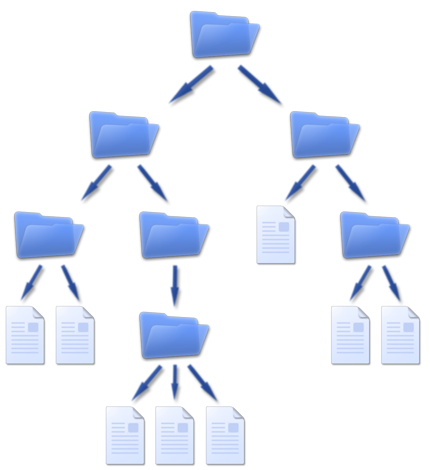
\includegraphics{https://personal.us.es/echevarria/Curso/images/FilesAndFolders.png}\\
\href{http://es.wikipedia.org/wiki/Archivo:FilesAndFolders.png}{Origen
de la imagen}

La estructura de directorios que sigue Linux es similar a la de
cualquier sistema UNIX. La estructura del sistema de archivos NO está
ligada de forma directa a la estructura de hardware. A diferencia de
Windows, es independiente del número de discos duros, disqueteras o
CDROMs. No hay una ``unidad'' para cada unidad física de disco o
partición como en Windows (**A:**,~**C:**, etc.), sino que todos los
discos duros o de red se montan bajo un sistema de directorios en árbol,
y algunos de esos directorios enlazan con estas unidades físicas de
disco. IMPORTANTE: Las barras en Linux al igual que en cualquier UNIX
son inclinadas hacia la derecha, como se puede ver más abajo (ese es el
motivo de que en internet sean inclinadas hacia la derecha, ya que nació
bajo UNIX).

\begin{itemize}
\item
  Estructura jerárquica de árbol invertido:
\item
  Desde una~\textbf{carpeta raiz}, denotada por~~/~, ``cuelgan'' otros
  archivos y/o carpetas.
\item
  De cada subcarpeta pueden ``colgar'' a su vez otros archivos y/o
  carpetas.
\item
  etc
\item
  ``Colgar'' significa~ ``estar contenido en''
\item
  Todos los archivos y/o carpetas están~ finalmente colgados de la
  carpeta raíz~~/
\item
  Carpeta ``\textbf{padre}'' de una carpeta es aquella que la contiene y
  está en el nivel inmediatamente superior de la estructura de árbol.
\end{itemize}

La ubicación de un fichero en la estructura de archivos se denota
mediante su~\textbf{path}~ó~\textbf{ruta}: se trata de una cadena de
caracteres que incluye todo el ``camino'' de directorios que llevan
desde el directorio raiz (~~/~~) hasta el fichero considerado. Se separa
un directorio del siguiente de nuevo mediante el caracter especial ~~/~~
.

Ejemplo: el path~~\textbf{/usr/local/bin/readme.txt}~~indica la
ubicación del fichero de nombre~~\textbf{readme.txt}~~que cuelga de la
carpeta~~\textbf{bin}~~que a su vez cuelga de la
carpeta~~\textbf{local}~~que a su vez cuelga de la
carpeta~~\textbf{usr}~~que cuelga de la raiz del sistema de archivos
~~/~~.

\textbf{ALGUNOS DIRECTORIOS IMPORTANTES}

Los directorios principales que podemos encontrar en cualquier sistema
Linux son:

Directorio

Descripción

\textbf{/}

Es la raíz del sistema de directorios. Aquí se monta la partición
principal Linux EXT.

\textbf{/etc}

Contiene los archivos de configuración de la mayoría de los programas.

\textbf{/home}

Contiene los archivos personales de los usuarios.

\textbf{/bin}

Contiene comandos básicos y muchos programas.

\textbf{/dev}

Contiene archivos simbólicos que representan partes del hardware, tales
como discos duros, memoria\ldots{}

\textbf{/mnt}

Contiene subdirectorios donde se montan (se enlaza con) otras
particiones de disco duro, CDROMs, etc.

\textbf{/tmp}

Ficheros temporales o de recursos de programas.

\textbf{/usr}

Programas y librerías instalados con la distribución

\textbf{/usr/local}

Programas y librerías instalados por el administrador

\textbf{/sbin}

Comandosadministrativos

\textbf{/lib}

Librerías varias y módulos (``trozos'') del kernel

\textbf{/var}

Datos varios como archivos de log (registro de actividad) de programas,
bases de datos, contenidos del servidor web, copias de seguridad\ldots{}

\textbf{/proc}

Información temporal sobre los procesos del sistema (explicaremos esto
más en profundidad posteriormente).

\textbf{OTROS CONCEPTOS RELACIONADOS CON DIRECTORIOS:}

\begin{itemize}
\item
  \textbf{Directorio}~o~\textbf{Carpeta de trabajo (Working Directory)}:
  es, en cada momento, el directorio en que se está trabajando.
  Cualquier fichero que el S.O. tenga que buscar, lo hará en primer
  lugar en dicho directorio.
\item
  \textbf{Ruta}~\textbf{(Path) de un fichero}: secuencia de directorios,
  separados por el símbolo~\textbf{/},~ que se ha de recorrer en la
  estructura de árbol para llegar a un fichero determinado.
\item
  \textbf{Path absoluto}: muestra toda la ruta desde la raiz del sistema
  de ficheros~\textbf{/}~~
\item
  \textbf{Path relativo}: muestra la ruta desde el directorio de
  trabajo.~ Puede empezar en:
\item
  una subdirectorio del directorio de trabajo,~ si el camino es
  descendente
\item
  \textbf{. .}~~si el camino comienza de forma ascendente
\item
  \textbf{.}~~ denota el directorio de trabajo
\item
  \textbf{. .}~~denota el directorio padre del directorio de trabajo
\item
  \textbf{Directorio o carpeta personal}~de un usuario (\textbf{home
  directory}): es el que contiene los ficheros de un usuario del
  sistema. Cada usuario tiene su propio directorio personal.
  Frecuentemente, los directorios personales cuelgan del
  directorio~\textbf{/home}, es decir, son de la
  forma~\textbf{/home/usuario}. Cuando se empieza una sesión en un
  sistema Linux, de forma automática se elige el~\textbf{home
  directory}~como~\textbf{working directory}.
\end{itemize}

\textbf{PUNTOS DE MONTAJE DE DISPOSITIVOS:}

En Linux, los distintos dispositivos conectados al ordenador forman
parte del sistema de archivos, de manera que, una vez montados, para el
usuario son como una carpeta más del sistema de ficheros. Habitualmente
se montan en~\textbf{/mnt}\\
Por ejemplo, la~\textbf{disquetera}~suele ser~~\textbf{/mnt/floppy}~~~ y
el~~\textbf{CDROM}~~ suele ser~~~\textbf{/mnt/cdrom}

\textbf{SISTEMAS DE ARCHIVOS COMPARTIDOS~Yellow Pages}

Este sistema permite que un conjunto de máquinas con sistemas Linux~
conectadas en red compartan un sistema de archivos común. Esto permite
que todos los usuarios de esas máquinas dispongan de todos sus archivos
en todas las máquinas. En este caso, el sistema de archivos suele estar
físicamente en una de las máquinas. Un usuario puede, así, acceder a
cualquiera de las máquinas con el mismo login y el mismo password.

Cuando se usa el servicio yellow pages (páginas amarillas), para cambiar
el password de un usuario es necesario utilizar el
comando~\textbf{yppasswd}~ en lugar de passwd.

PROPIEDAD, PERMISOS Y DERECHOS DE ACCESO A CARPETAS Y FICHEROS

Al ser Linux un sistema multiusuario, es preciso que esté definido de
quién es cada cosa (carpetas y ficheros) y qué derechos de acceso tiene
cada usuario.

Cada usuario es propietario, en general, de todos los ficheros y
subdirectorios que cuelgan de su directorio personal: puede crear,
modificar y borrar en él todo lo que quiera. Ningún otro usuario
(excepto el root) puede acceder~a los ficheros de otro, ni siquiera
verlos.

En Linux, cada fichero y carpeta tiene
un~\textbf{propietario}~(\textbf{owner}). El propietario es el que
define los permisos de acceso de otros usuarios a sus ficheros. Para
ello, el conjunto de usuarios de una máquina se entiende dividido en
tres grupos:

\begin{itemize}
\tightlist
\item
  el mismo propietario (\textbf{owner})
\item
  el grupo de usuarios al que pertenece el propietario (\textbf{group})
\item
  el resto del mundo (\textbf{world})
\end{itemize}

Dichos permisos, a su vez, son de tres tipos:

\begin{itemize}
\tightlist
\item
  de lectura (\textbf{read})
\item
  de escritura (\textbf{write})
\item
  de ejecución (\textbf{execute})
\end{itemize}

Los permisos de acceso a un fichero sólo los puede cambiar el
propietario y el (todopoderoso)~\textbf{root}. En general, cada usuario
puede leer en el resto de directorios del sistema de ficheros, excepto
en la del root y en las de los otros usuarios.

\begin{itemize}
\tightlist
\item
  Los ficheros y carpetas del sistema son propiedad del root
\item
  Los ficheros y carpetas de programas instalados son propiedad del~
  root
\item
  El~ root tiene todos los permisos sobre todos los ficheros de todos
  los usuarios.
\end{itemize}

EL GESTOR DE VENTANAS KDE

\textbf{PANTALLA KDE:}

\begin{quote}
\textbf{Panel de KDE:}

\begin{itemize}
\tightlist
\item
  Menú de inicio de aplicaciones
\item
  Escritorios virtuales
\item
  Directorio Personal
\item
  Lista de ventanas abiertas
\item
  Emulador de Terminal
\item
  Editores sencillos: Kedit, Kwrite
\end{itemize}
\end{quote}

\begin{quote}
\textbf{Ventanas:}

\begin{itemize}
\item
  Barra de títulos:
\item
  Icono de aplicación (Manipulación de ventanas)
\item
  Fijación de ventana
\item
  Minimizar, maximizar y cerrar
\item
  Barra de menús
\item
  Barra de herramientas
\end{itemize}
\end{quote}

\begin{quote}
\textbf{Konqueror: Gestor gráfico de archivos (File Manager):}

\begin{itemize}
\tightlist
\item
  Navegar por la estructura de directorios
\item
  Crear y borrar carpetas
\item
  Copiar y mover carpetas
\item
  Cambiar nombre a ficheros y carpetas
\item
  Abrir y borrar ficheros
\item
  Ver y modificar las propiedades de ficheros y carpetas
\end{itemize}
\end{quote}

\begin{quote}
\textbf{Konsole: Emulador de terminal}

Se usa para trabajar con el Sistema Operativo en modo de comandos, es
decir para introducir directamente instrucciones UNIX al sistema. Las
instrucciones se escriben en la Línea de Comandos, después
del~\textbf{prompt}~del usuario.
\end{quote}

\textbf{ALGUNOS COMANDOS:}

\begin{quote}
\textbf{clear}

limpia la pantalla

\textbf{date}

devuelve la fecha y hora actuales

\textbf{cal}

muestra el calendario

\textbf{history}

muestra la historia de los últimos comandos usados

\textbf{man comando}

Muestra la página del manual correspondiente al comando

\textbf{more file}

Si~\textbf{file}~es un fichero de texto, lo muestra de página en página.
Se pasa página con la barra espaciadora. Se termina con~\textbf{q}

\textbf{ls}

muestra el contenido del directorio de trabajo

\textbf{ls -l}

muestra el contenido del directorio de trabajo en forma de lista,
incluyendo información extra

\textbf{ls -a}

muestra el contenido del directorio de trabajo incluídos los ficheros
ocultos

\textbf{ls dir}

ejecuta~\textbf{ls}~sobre el directorio~\textbf{dir}~- se pueden usar
opciones:~\textbf{ls -la dir}

\textbf{pwd}

muestra el nombre del directorio de trabajo (print working directory)

\textbf{df}

muestra el espacio libre y usado en los discos

\textbf{du -sk dir}

muestra la cantidad de espacio de disco usada por el
directorio~\textbf{dir}~(y todo lo que hay dentro)

\textbf{du -Sk dir}

lo mismo, pero especificando por subdirectorios

\textbf{mkdir name}

crea un directorio de nombre~\textbf{name}~(make directory) -
si~\textbf{name}~no incluye un~\textbf{path}, el directorio se crea en
el directorio de trabajo

\textbf{rm fich}

borra el fichero~\textbf{fich}~(remove)

\textbf{rmdir direc}

borra el directorio~~\textbf{dir}~(tiene que estar vacío)

\textbf{rm -i fich}

antes de borrar el fichero~\textbf{fich}, pide confirmación (modo
interactivo)

\textbf{cp fich dir}

crea una copia del fichero~\textbf{fich}~en el directorio~\textbf{dir}

\textbf{cp fich1 fich2}

crea una copia del fichero~\textbf{fich1}~y le pone el
nombre~\textbf{fich2}

\textbf{mv fich dir}

``mueve'' el fichero~\textbf{fich}~~al directorio~\textbf{dir}

\textbf{mv fich1 fich2}

``mueve'' el fichero~\textbf{fich1}~~al fichero~\textbf{fich2}~(es
decir, lo cambia de nombre) (\textbf{fich2}~puede también incluir
un~\textbf{path}; en ese caso también lo cambia de sitio)

\textbf{cd}

cambia el directorio de trabajo al directorio personal (home)

\textbf{cd dir}

cambia el directorio de trabajo al directorio~\textbf{dir}

\textbf{cd ..}

cambia el directorio de trabajo al ``padre'' del actual

\textbf{ps}

proporciona información sobre los procesos activos del usuario

\textbf{ps aux}

proporciona información sobre todos los procesos activos en el sistema

\textbf{kill -9 PID}

elimina el proceso con número de identificación PID

\textbf{gzip fich}

crea un fichero de nombre~\textbf{fich.gz}, comprimido de~\textbf{fich}

\textbf{gunzip fich.gz}

descomprime el fichero~\textbf{fich.gz}

\textbf{tar}

condensa directorios en un sólo fichero y viceversa

\textbf{tar -cf file.tar direc}

crea el fichero~\textbf{file.tar}~con el contenido del
directorio~\textbf{direc}

\textbf{tar -cvf file.tar direc}

lo mismo, pero con explicaciones (v==verbose)

\textbf{tar -xf file.tar}

extrae los ficheros de~\textbf{file.tar}

\textbf{tar -xvf file.tar}

los mismo, pero con explicaciones

\textbf{exit}

finaliza la sesión de trabajo; en un terminal, cierra el terminal.
\end{quote}

\textbf{PERSONALIZACIÓN DE LAS CUENTAS:}

\begin{quote}
\begin{itemize}
\tightlist
\item
  el fichero de configuración~\textbf{.bashrc}
\item
  definición o modificación de comandos:~\textbf{alias}
\item
  variable de entorno~\textbf{PATH}: definición de los caminos de
  búsqueda
\item
  ejecución de un fichero de configuración:~\textbf{source}
\end{itemize}
\end{quote}

\textbf{MODIFICACIÓN DEL FICHERO DE CONFIGURACIÓN .bahsrc PARA EL ACENTO
\^{} EN MATLAB:}

\begin{quote}
\begin{itemize}
\tightlist
\item
  En el directorio personal, editar el fichero oculto~\textbf{.bashrc}
\item
  Añadir, al final, la orden:~\textbf{setxkbmap -variant nodeadkeys}
\end{itemize}
\end{quote}


\printbibliography


\end{document}
